\tikzstyle{vertex}=[circle,fill=black!25,minimum size=20pt,inner sep=0pt]
\tikzstyle{novertex}=[]
\tikzstyle{smallvertex}=[circle,fill=black,minimum size=6pt,inner sep=0pt]
\tikzstyle{edge} = [draw,thin,->]
\tikzstyle{weight} = [font=\small]
\tikzstyle{selected edge} = [draw,line width=3pt,-,red!50]
\tikzstyle{big edge} = [draw,line width=2pt,->,black]
\tikzstyle{cutting edge} = [draw,line width=3pt,-,red]
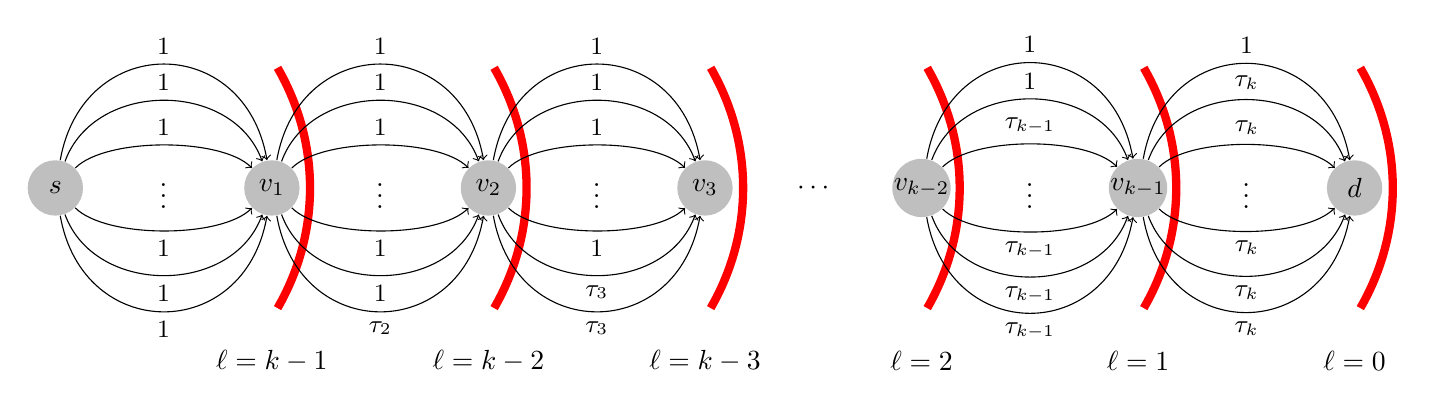
\begin{tikzpicture}[scale=0.55,auto,swap]
    \node[vertex](s1) at (0,0){$s$};
    \node[vertex](s2) at (5,0){$v_1$};
    \node[novertex](s2o) at (5,3){};
    \node[novertex](s2u) at (5,-3){};
    \node[novertex](s2t) at (5,-4){$\ell=k-1$};

    \node[vertex](s3) at (10,0){$v_2$};
    \node[novertex](s3o) at (10,3){};
    \node[novertex](s3u) at (10,-3){};
    \node[novertex](s3t) at (10,-4){$\ell=k-2$};
    
    \node[vertex](s35) at (15,0){$v_3$};
    \node[novertex](s35o) at (15,3){};
    \node[novertex](s35u) at (15,-3){};
    \node[novertex](s35t) at (15,-4){$\ell=k-3$};
    
    \node[vertex](s4) at (20,0){$v_{k-2}$};
    \node[novertex](s4o) at (20,3){};
    \node[novertex](s4u) at (20,-3){};
    \node[novertex](s4t) at (20,-4){$\ell=2$};
    
    \node[vertex](s5) at (25,0){$v_{k-1}$};
    \node[novertex](s5o) at (25,3){};
    \node[novertex](s5u) at (25,-3){};
    \node[novertex](s5t) at (25,-4){$\ell=1$};
    
    \node[vertex](t) at (30,0){$d$};
    \node[novertex](to) at (30,3){};
    \node[novertex](tu) at (30,-3){};
    \node[novertex](tt) at (30,-4){$\ell=0$};

    \draw [edge] (s1) to[out=80,in=100, distance=3cm ] node[weight,above,black]{$1$} (s2);
    \draw [edge] (s1) to[out=70,in=110, distance=2cm ] node[weight,above,black]{$1$} (s2);
    \draw [edge] (s1) to[out=45,in=135, distance=1cm ] node[weight,above,black]{$1$} (s2);
    \node[text width=0.1cm] at (2.5,0) {$\vdots$};
    \draw [edge] (s1) to[out=-45,in=-135, distance=1cm ] node[weight,below,black]{$1$} (s2);
    \draw [edge] (s1) to[out=-70,in=-110, distance=2cm ] node[weight,below,black]{$1$} (s2);
    \draw [edge] (s1) to[out=-80,in=-100, distance=3cm ] node[weight,below,black]{$1$} (s2);

    \draw [cutting edge] (s2o) to[out=-60,in=60, distance=2cm ] node[weight,below,black]{} (s2u);    

    \draw [edge] (s2) to[out=80,in=100, distance=3cm ] node[weight,above,black]{$1$} (s3);
    \draw [edge] (s2) to[out=70,in=110, distance=2cm ] node[weight,above,black]{$1$} (s3);
    \draw [edge] (s2) to[out=45,in=135, distance=1cm ] node[weight,above,black]{$1$} (s3);
    \node[text width=0.1cm] at (7.5,0) {$\vdots$};
    \draw [edge] (s2) to[out=-45,in=-135, distance=1cm ] node[weight,below,black]{$1$} (s3);
    \draw [edge] (s2) to[out=-70,in=-110, distance=2cm ] node[weight,below,black]{$1$} (s3);
    \draw [edge] (s2) to[out=-80,in=-100, distance=3cm ] node[weight,below,black]{$\tau_2$} (s3);

    \draw [cutting edge] (s3o) to[out=-60,in=60, distance=2cm ] node[weight,below,black]{} (s3u); 

    \draw [edge] (s3) to[out=80,in=100, distance=3cm ] node[weight,above,black]{$1$} (s35);
    \draw [edge] (s3) to[out=70,in=110, distance=2cm ] node[weight,above,black]{$1$} (s35);
    \draw [edge] (s3) to[out=45,in=135, distance=1cm ] node[weight,above,black]{$1$} (s35);
    \node[text width=0.1cm] at (12.5,0) {$\vdots$};
    \draw [edge] (s3) to[out=-45,in=-135, distance=1cm ] node[weight,below,black]{$1$} (s35);
    \draw [edge] (s3) to[out=-70,in=-110, distance=2cm ] node[weight,below,black]{$\tau_3$} (s35);
    \draw [edge] (s3) to[out=-80,in=-100, distance=3cm ] node[weight,below,black]{$\tau_3$} (s35);

    \draw [cutting edge] (s35o) to[out=-60,in=60, distance=2cm ] node[weight,below,black]{} (s35u);
    
    \node[] at (17.5,0) {$\cdots$};

    \draw [cutting edge] (s4o) to[out=-60,in=60, distance=2cm ] node[weight,below,black]{} (s4u);
    
    \draw [edge] (s4) to[out=80,in=100, distance=3cm ] node[weight,above,black]{$1$} (s5);
    \draw [edge] (s4) to[out=70,in=110, distance=2cm ] node[weight,above,black]{$1$} (s5);
    \draw [edge] (s4) to[out=45,in=135, distance=1cm ] node[weight,above,black]{$\tau_{k-1}$} (s5);
    \node[text width=0.1cm] at (22.5,0) {$\vdots$};
    \draw [edge] (s4) to[out=-45,in=-135, distance=1cm ] node[weight,below,black]{$\tau_{k-1}$} (s5);
    \draw [edge] (s4) to[out=-70,in=-110, distance=2cm ] node[weight,below,black]{$\tau_{k-1}$} (s5);
    \draw [edge] (s4) to[out=-80,in=-100, distance=3cm ] node[weight,below,black]{$\tau_{k-1}$} (s5);

    \draw [cutting edge] (s5o) to[out=-60,in=60, distance=2cm ] node[weight,below,black]{} (s5u);    

    \draw [edge] (s5) to[out=80,in=100, distance=3cm ] node[weight,above,black]{$1$} (t);
    \draw [edge] (s5) to[out=70,in=110, distance=2cm ] node[weight,above,black]{$\tau_k$} (t);
    \draw [edge] (s5) to[out=45,in=135, distance=1cm ] node[weight,above,black]{$\tau_k$} (t);
    \node[text width=0.1cm] at (27.5,0) {$\vdots$};
    \draw [edge] (s5) to[out=-45,in=-135, distance=1cm ] node[weight,below,black]{$\tau_k$} (t);
    \draw [edge] (s5) to[out=-70,in=-110, distance=2cm ] node[weight,below,black]{$\tau_k$} (t);
    \draw [edge] (s5) to[out=-80,in=-100, distance=3cm ] node[weight,below,black]{$\tau_k$} (t);

    \draw [cutting edge] (to) to[out=-60,in=60, distance=2cm ] node[weight,below,black]{} (tu);
    
 \end{tikzpicture}

 